%==============================================================================
% figures/F1_tail_equivalence.tex --- Implementation placeholder
%==============================================================================
% Required source CSV: results/F1_tail_equivalence.csv
% Required columns: seed, spawned_seed, N, alpha, x, n, mu_hat, ci_low, ci_high, first_order, second_order, truth_method
% Target diagnostic: Plot log-log tail estimates against first- and second-order asymptotics.
% Replacement instruction:
%   Generate a PDF/PNG with the same basename and replace the tikzpicture below
%   by 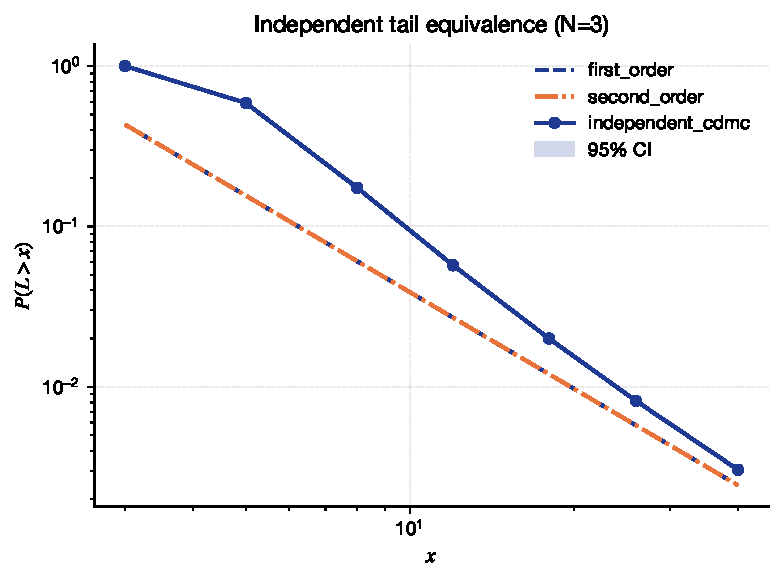
\includegraphics[width=0.85\linewidth]{figures/F1_tail_equivalence.pdf}.
%==============================================================================
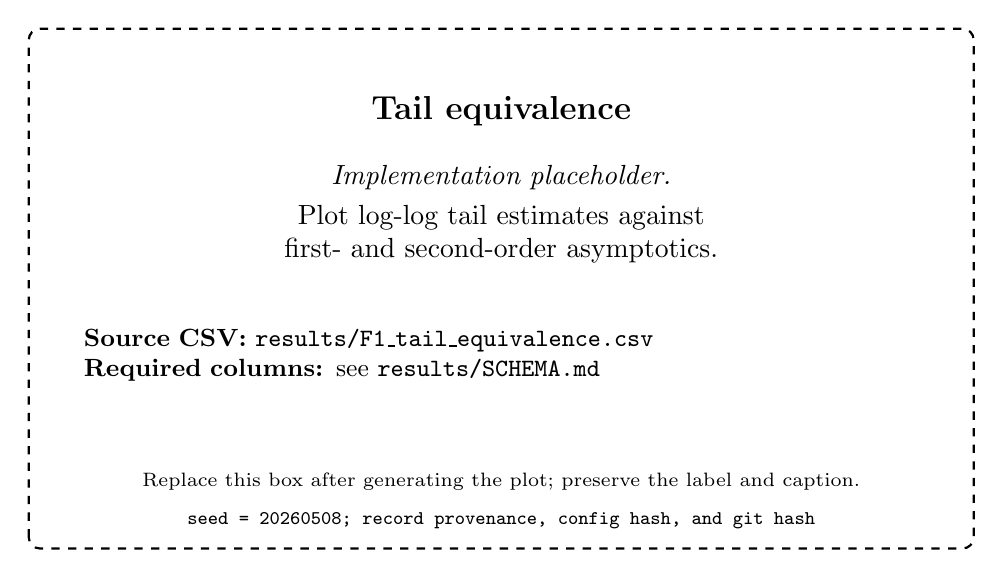
\begin{tikzpicture}
\draw[thick, dashed, rounded corners] (0,0) rectangle (12,6.6);
\node[align=center, font=\large] at (6,5.55) {\textbf{Tail equivalence}};
\node[align=center, text width=10.6cm] at (6,4.25) {\emph{Implementation placeholder.}\\[0.25em]
Plot log-log tail estimates against first- and second-order asymptotics.};
\node[align=left, text width=10.6cm, font=\small] at (6,2.45) {\textbf{Source CSV:} \texttt{results/F1\_tail\_equivalence.csv}\\
\textbf{Required columns:} see \texttt{results/SCHEMA.md}};
\node[align=center, font=\scriptsize] at (6,0.85) {Replace this box after generating the plot; preserve the label and caption.};
\node[align=center, font=\scriptsize\ttfamily] at (6,0.35) {seed = 20260508; record provenance, config hash, and git hash};
\end{tikzpicture}
